%package list
\documentclass{article}
\usepackage[top=3cm, bottom=3cm, outer=3cm, inner=3cm]{geometry}
\usepackage{graphicx}
\usepackage{url}

%% \usepackage{cite}
\usepackage{hyperref}
\usepackage{array}
\usepackage{multicol}
\newcolumntype{x}[1]{>{\centering\arraybackslash\hspace{0pt}}p{#1}}
\usepackage{natbib}
\usepackage{pdfpages}
\usepackage{multirow}
\usepackage{float}
\usepackage[normalem]{ulem}
\useunder{\uline}{\ul}{}


%%%%%%%%%%%%%%%%%%%%%%%%%%%%%%%%%%%%%%%%%%%%%%%%%%%%%%%%%%%%%%%%%%%%%%%%%%%%
%%%%%%%%%%%%%%%%%%%%%%%%%%%%%%%%%%%%%%%%%%%%%%%%%%%%%%%%%%%%%%%%%%%%%%%%%%%%
\newcommand{\csemail}{vmachacaa@unsa.edu.pe}
\newcommand{\csdocente}{Vicente Machaca Arceda}
\newcommand{\cscurso}{Algoritmos y Estructura de Datos}
\newcommand{\csuniversidad}{Universidad Nacional de San Agustín}
\newcommand{\csescuela}{Maestría en Ciencia de la Computación}
\newcommand{\cspracnr}{02}
\newcommand{\cstema}{--}
%%%%%%%%%%%%%%%%%%%%%%%%%%%%%%%%%%%%%%%%%%%%%%%%%%%%%%%%%%%%%%%%%%%%%%%%%%%%
%%%%%%%%%%%%%%%%%%%%%%%%%%%%%%%%%%%%%%%%%%%%%%%%%%%%%%%%%%%%%%%%%%%%%%%%%%%%


\usepackage[english,spanish]{babel}
\usepackage[utf8]{inputenc}
\AtBeginDocument{\selectlanguage{spanish}}
\renewcommand{\figurename}{Figura}
\renewcommand{\refname}{Referencias}
\renewcommand{\tablename}{Tabla} %esto no funciona cuando se usa babel
\AtBeginDocument{%
	\renewcommand\tablename{Tabla}
}

\usepackage{fancyhdr}
\pagestyle{fancy}
\fancyhf{}
\setlength{\headheight}{30pt}
\renewcommand{\headrulewidth}{1pt}
\renewcommand{\footrulewidth}{1pt}
\fancyhead[L]{\raisebox{-0.2\height}{
\includegraphics[width=3cm]{img/logo_unsa.jpg}}}
\fancyhead[C]{}
\fancyhead[R]{\fontsize{7}{7}\selectfont	\csuniversidad \\ \csescuela \\ \textbf{\cscurso} }
\fancyfoot[L]{MSc. Vicente Machaca}
\fancyfoot[C]{\cscurso}
\fancyfoot[R]{Página \thepage}

\begin{document}
	
	\vspace*{10px}
	
	\begin{center}	
		\fontsize{17}{17} \textbf{ Práctica \cspracnr}
	\end{center}
	%\centerline{\textbf{\underline{\Large Título: Informe de revisión del estado del arte}}}
	%\vspace*{0.5cm}
	

	\begin{table}[h]
		\begin{tabular}{|x{4.7cm}|x{4.8cm}|x{4.8cm}|}
			\hline 
			\textbf{DOCENTE} & \textbf{CARRERA}  & \textbf{CURSO}   \\
			\hline 
			\csdocente & \csescuela & \cscurso    \\
			\hline 
		\end{tabular}
	\end{table}	
	
	
	\begin{table}[h]
		\begin{tabular}{|x{4.7cm}|x{4.8cm}|x{4.8cm}|}
			\hline 
			\textbf{PRÁCTICA} & \textbf{TEMA}  & \textbf{DURACIÓN}   \\
			\hline 
			\cspracnr & Estructuras de datos & 3 horas   \\
			\hline 
		\end{tabular}
	\end{table}
	
	
	\section{Datos de los estudiantes}
	\begin{itemize}
		\item Grupo: V
		\item Integrantes: 
		\begin{itemize}
			\item Angel Yvan Choquehuanca Peraltilla
			\item Estefany Pilar Huaman Colque
            \item Eduardo Diaz Huayhuas
            \item Gustavo Raul Manrique Fernandez
		\end{itemize}		
	\end{itemize}
	
	
 
	
	%\clearpage
	%\bibliographystyle{apalike}
	%\bibliographystyle{IEEEtranN}
	%\bibliography{bibliography}
		

    \section{Introducción}
    En el caso de árboles binarios, si los árboles están sesgados, se vuelven computacionalmente ineficientes para realizar operaciones en ellos.
    Esta es la motivación detrás de asegurarse de que los árboles no estén sesgados. De ahí la necesidad de árboles binarios balanceados.

    
    \section{Marco Teorico}
Árbol de búsqueda binario autoequilibrado

	
		\subsection{Estructura de datos AVL}
		
Un árbol AVL es un árbol de búsqueda binario balanceado. En un árbol AVL, el factor de equilibrio de cada nodo es -1, 0 o +1.

El factor de equilibrio de un nodo es la diferencia entre las alturas de los subárboles izquierdo y derecho de ese nodo. El factor de equilibrio de un nodo se calcula ya sea altura del subárbol izquierdo - altura del subárbol derecho (O) altura del subárbol derecho - altura del subárbol izquierdo . En la siguiente explicación, calculamos de la siguiente manera:

 \fbox{Factor de equilibrio = altura del subárbol izquierdo - altura del subárbol derecho}

En el árbol AVL, después de realizar operaciones como inserción y eliminación, debemos verificar el factor de equilibrio de cada nodo en el árbol. Si todos los nodos satisfacen la condición del factor de equilibrio, concluimos la operación; de lo contrario, debemos equilibrarlo. Cada vez que el árbol se desequilibra debido a alguna operación, utilizamos operaciones de rotación para equilibrar el árbol.La rotación es el proceso de mover los nodos hacia la izquierda o hacia la derecha para equilibrar el árbol.

Hay cuatro rotaciones y se clasifican en dos tipos:

\begin{itemize}
   \item Rotación izquierda
   \item Rotación a la derecha
   \item Rotación izquierda-derecha
   \item Rotación derecha-izquierda
\end{itemize}	


\begin{enumerate}

		\item \textbf{Rotación Simple a la izquierda (rotación LL)}
		En Rotación LL, cada nodo se mueve una posición a la izquierda desde la posición actual. Para comprender la Rotación LL, consideremos la siguiente operación de inserción en el Árbol AVL.
		
		\begin{figure}[H]
\centering
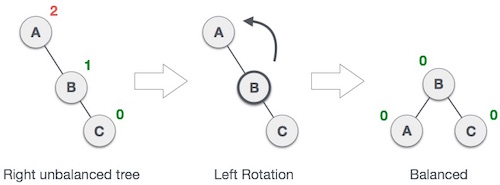
\includegraphics[width=0.9\textwidth]{img/avl_left_rotation.jpg}
\caption{Rotación LL}
\end{figure}
		
		\item \textbf{Rotación Simple a la derecha (rotación RR)}
		n Rotación RR, cada nodo se mueve una posición a la derecha desde la posición actual. Para comprender la rotación RR, consideremos la siguiente operación de inserción en el árbol AVL.
		
		\begin{figure}[H]
\centering
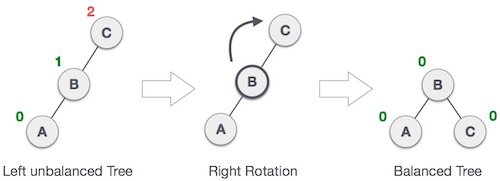
\includegraphics[width=0.9\textwidth]{img/avl_right_rotation.jpg}
\caption{Rotación RR}
\end{figure}
		
		\item \textbf{Rotación izquierda derecha (rotación LR)}
		La rotación LR es una secuencia de una sola rotación a la izquierda seguida de una sola rotación a la derecha. En LR Rotation, al principio, cada nodo se mueve una posición a la izquierda y una posición a la derecha desde la posición actual. Para comprender la Rotación LR, consideremos la siguiente operación de inserción en el Árbol AVL.
		
		\begin{figure}[H]
\centering
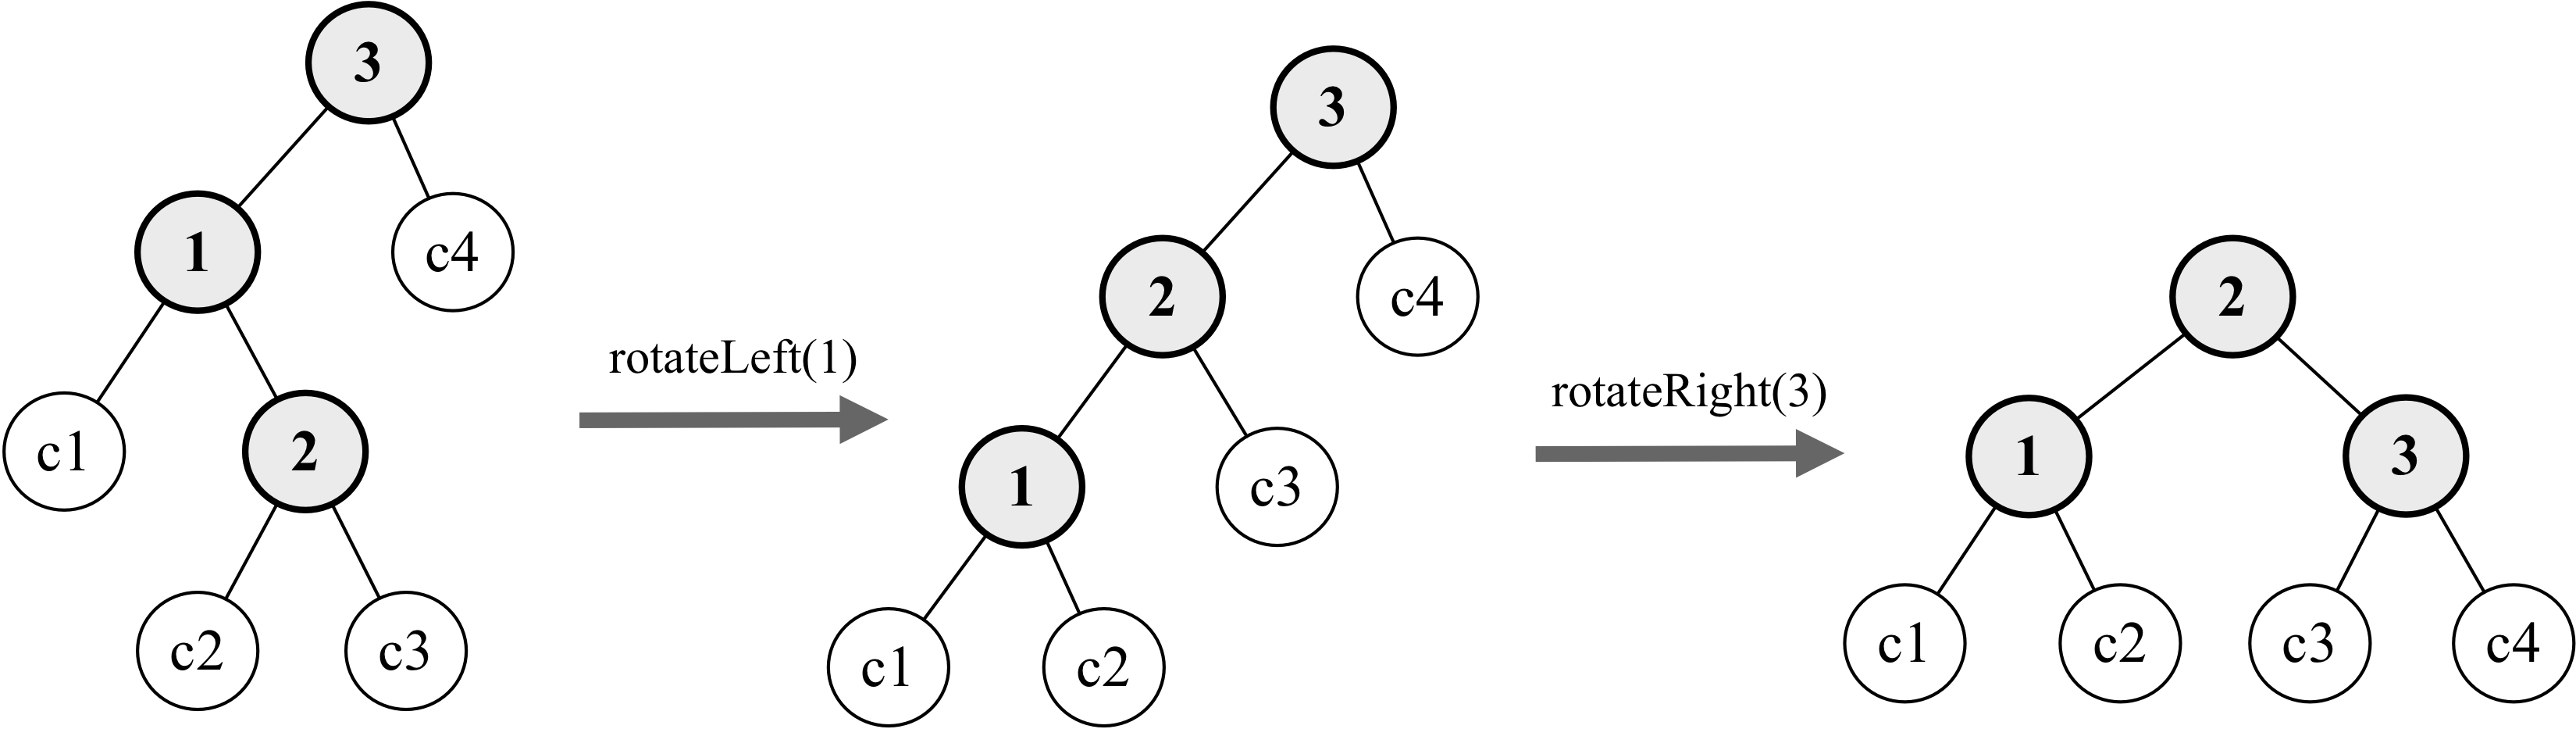
\includegraphics[width=0.9\textwidth]{img/Rotation_Complex_AVL.png}
\caption{Rotación LR}
\end{figure}
		
		\item \textbf{Rotación derecha izquierda (rotación RL)}
		La rotación RL es una secuencia de una sola rotación a la derecha seguida de una sola rotación a la izquierda. En Rotación RL, al principio cada nodo se mueve una posición a la derecha y una posición a la izquierda desde la posición actual. Para comprender la Rotación RL, consideremos la siguiente operación de inserción en el Árbol AVL.
		\end{enumerate}
	\begin{figure}[H]
\centering
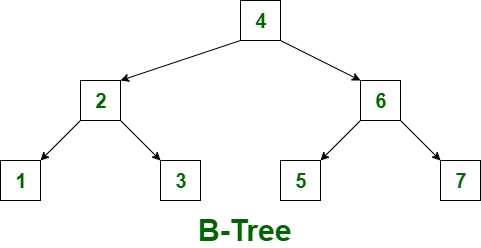
\includegraphics[width=0.9\textwidth]{img/B-Tree.png}
\caption{Rotación RL}
\end{figure}		
		
Las siguientes operaciones se realizan en el árbol AVL:

	\begin{enumerate}

		\item \textbf{Operación Búsqueda}
	En un árbol AVL, la operación de búsqueda se realiza con una complejidad de tiempo O(log n) . La operación de búsqueda en el árbol AVL es similar a la operación de búsqueda en un árbol de búsqueda binario. Usamos los siguientes pasos para buscar un elemento en el árbol AVL:
		
		\begin{itemize}
		\item Paso 1: lee el elemento de búsqueda del usuario.
		\item Paso 2: compare el elemento de búsqueda con el valor del nodo raíz en el árbol.
		\item Paso 3: Si ambos no coinciden, verifica si el elemento de búsqueda es más pequeño o más grande que el valor de ese nodo.
		\item Paso 4: si el elemento de búsqueda es más pequeño, continúa el proceso de búsqueda en el subárbol izquierdo.
		\item Paso 5: si el elemento de búsqueda es más grande, continúa el proceso de búsqueda en el subárbol derecho.
		\item Paso 6: Repite lo mismo hasta encontrar el elemento exacto o hasta comparar el elemento de búsqueda con el nodo hoja.
		\item Paso 7: si llega al nodo que tiene el valor igual al valor de búsqueda y finaliza la función.
		\item Paso 8: si llega al nodo de hoja y tampoco coincide con el elemento de búsqueda, finaliza la función.
		\end{itemize}


		\item \textbf{Operación Inserción}
		En un árbol AVL, la operación de inserción se realiza con una complejidad de tiempo O(log n) . En AVL Tree, siempre se inserta un nuevo nodo como un nodo hoja. La operación de inserción se realiza de la siguiente manera:
		\begin{itemize}
		\item Paso 1: inserte el nuevo elemento en el árbol utilizando la lógica de inserción del árbol de búsqueda binaria.
		\item Paso 2: después de la inserción,se verifica el factor de equilibrio de cada nodo.
		\item Paso 3: si el factor de equilibrio de cada nodo es 0, 1 o -1 , va a la siguiente operación.
		\item Paso 4: si el factor de equilibrio de cualquier nodo es distinto de 0, 1 o -1 , se dice que ese árbol está desequilibrado. En este caso, realiza la Rotación adecuada para equilibrarlo y va a la siguiente operación.
				\end{itemize}
				
		\item \textbf{Operación Eliminación}
				La operación de eliminación en AVL Tree es similar a la operación de eliminación en BST. Pero después de cada operación de eliminación, debemos verificar la condición del factor de equilibrio. Si el árbol está equilibrado después de la eliminación, vaya a la siguiente operación; de lo contrario, realice una rotación adecuada para equilibrar el árbol.
			\end{enumerate}
		
		

		\subsection{Estructura de datos B Tree}

B-Tree es un árbol de búsqueda autoequilibrado en el que cada nodo contiene varias claves y tiene más de dos elementos secundarios. Donde el número de claves en un nodo y el número de hijos para un nodo depende del orden de B-Tree. Cada B-Tree tiene un orden.

B-Tree de Orden m tiene las siguientes propiedades:
\begin{itemize}
   \item Propiedad n.º 1 : todos los nodos de hoja deben estar al mismo nivel .
   \item Propiedad n.º 2 : todos los nodos, excepto el raíz, deben tener al menos [m/2]-1 claves y un máximo de m-1 claves.
   \item Propiedad n.º 3 : todos los nodos que no son hojas excepto la raíz (es decir, todos los nodos internos) deben tener al menos m/2 hijos.
   \item Propiedad n.º 4 : si el nodo raíz no es un nodo hoja, debe tener al menos 2 hijos.
   \item Propiedad n.º 5 : un nodo que no sea hoja con n-1 claves debe tener n número de hijos.
   \item Propiedad n.º 6 : todos los valores clave de un nodo deben estar en orden ascendente .
\end{itemize}


\begin{figure}[H]
\centering
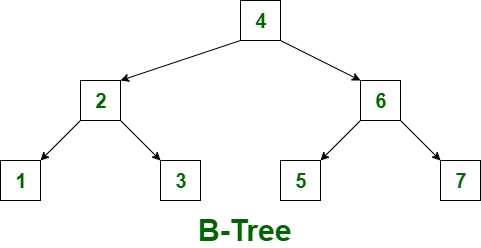
\includegraphics[width=0.9\textwidth]{img/B-Tree.png}
\caption{Ejemplo de Estructura de datos B Tree}
\end{figure}


Las siguientes operaciones se realizan en un B-Tree:

	\begin{enumerate}

		\item \textbf{Operación Búsqueda}
		La operación de búsqueda en B-Tree es similar a la operación de búsqueda en Binary Search Tree. En un árbol de búsqueda binario, el proceso de búsqueda comienza desde el nodo raíz y tomamos una decisión bidireccional cada vez (vamos al subárbol izquierdo o al subárbol derecho). En B-Tree también el proceso de búsqueda comienza desde el nodo raíz, pero aquí siempre tomamos una decisión de n vías. Donde 'n' es el número total de hijos que tiene el nodo. En un B-Tree, la operación de búsqueda se realiza con una complejidad de tiempo O(log n) . La operación de búsqueda se realiza de la siguiente manera:
		
		\begin{itemize}
		\item Paso 1: lee el elemento de búsqueda del usuario.
		\item Paso 2: compara el elemento de búsqueda con el primer valor clave del nodo raíz en el árbol. 
		\item Paso 3: si ambos coinciden, se muestra el nodo encontrado y termina la función.
		\item Paso 4: si ninguno de los dos coincide, comprueba si el elemento de búsqueda es más pequeño o más grande que el valor de la clave.
		\item Paso 5: si el elemento de búsqueda es más pequeño, continúa el proceso de búsqueda en el subárbol izquierdo.
		\item Paso 6: si el elemento de búsqueda es más grande, compara el elemento de búsqueda con el siguiente valor clave en el mismo nodo y repite los pasos 3, 4, 5 y 6 hasta que encontrar la coincidencia exacta o hasta que el elemento de búsqueda se compare con el último valor clave en el nodo hoja.
		\item Paso 7: si el último valor clave en el nodo hoja tampoco coincide, finalice la función.
		\end{itemize}


			\item \textbf{Operación Inserción}
			En un B-Tree, se debe agregar un nuevo elemento solo en el nodo hoja. Eso significa que el nuevo valor clave siempre se adjunta solo al nodo hoja. La operación de inserción se realiza de la siguiente manera:
			
		
\begin{itemize}
\item Paso 1: comprueba si el árbol está vacío.
 \item Paso 2: si el árbol está vacío , crea un nuevo nodo con un nuevo valor de clave y lo inserta en el árbol como un nodo raíz.
\item Paso 3: si el árbol no está vacío , busca el nodo de hoja adecuado al que se agrega el nuevo valor clave utilizando la lógica del árbol de búsqueda binaria.
\item Paso 4: si ese nodo hoja tiene una posición vacía, agrega el nuevo valor clave a ese nodo hoja en orden ascendente de valor clave dentro del nodo.
\item Paso 5: si ese nodo de hoja ya está lleno, divide ese nodo de hoja enviando el valor medio a su nodo principal. Repite lo mismo hasta que el valor de envío se fije en un nodo.
\item Paso 6: si el derrame se realiza en el nodo raíz, el valor medio se convierte en un nuevo nodo raíz para el árbol y la altura del árbol aumenta en uno.
\end{itemize}
\end{enumerate}
    \section{Metodologia y Desarrollo}
    \subsection{Codigo Fuente}
    Para el desarrollo del  codigo se utilizó el lenguaje \href{https://www.javascript.com/}{JavaScript}, donde se utiliza la libreria \href{https://p5js.org/es/}{p5.js}
    \subsection{Despliegue en la nube}
    Para la realización de este proyecto, se utilizó los servicios en la nube de Heroku \href{https://www.heroku.com/}{www.heroku.com}, bajo la direcciones:

    \begin{itemize}
        \item B-Tree: \href{https://mcc-project2-group5-btree.herokuapp.com/}{Heroku B-Tree}
        \item AVL-Tree: \href{https://mcc-project2-group5-avl.herokuapp.com/}{Heroku AVL-Tree}
    \end{itemize}

	El repositorio donde se encuentran los archivos fuente se encuentra en: \href{https://github.com/AngelYvan/mcc-proyecto2-grupo5}{Github - MCC - Proyecto 2}
    	
	\subsection{Ejecución del Programa}
    \subsubsection{B-Tree}
    Para el B-Tree se tiene un panel en la izquierda donde se puede hacer las operaciones siguientes:
    \begin{itemize}
        \item Insert (Insertar)
        \item Search (Buscar)
        \item Delete (Borrar)
    \end{itemize}
    
        \begin{figure}[H]
        \centering
        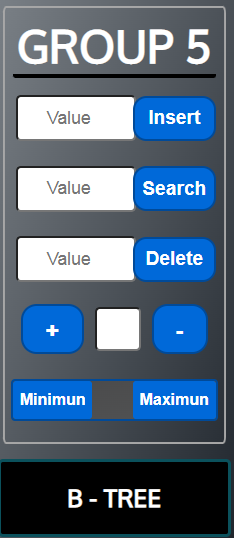
\includegraphics[width=0.2\textwidth]{img/btree_cap1.PNG}
        \caption{Panel de Control de B-Tree}
        \end{figure}

    Se deben colocar los datos en las cajas respectivas y hacer clic en la operación que se desea realizar. 
    Luego se visualiza la formación del arbol en la parte derecha de la aplicación.

        \begin{figure}[H]
        \centering
        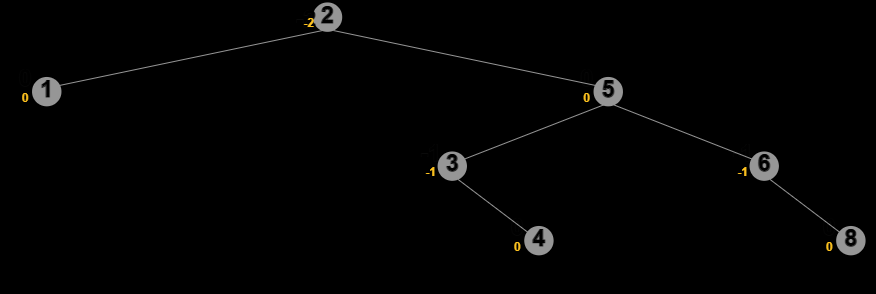
\includegraphics[width=0.8\textwidth]{img/btree_arbol.PNG}
        \caption{Formacion del arbol B-Tree}
        \end{figure}

    Si hay una duplicación el programa en el Status Bar mostrará un error:

        \begin{figure}[H]
        \centering
        
\includegraphics[width=0.6\textwidth]{img/btree_alreadyexist.PNG}
        \caption{Error de Existencia}
        \end{figure}

En el caso que no exista el dato, se procede a insertar y se muestra el mensaje siguiente:

        \begin{figure}[H]
        \centering
        
\includegraphics[width=0.6\textwidth]{img/btree_insertok.PNG}
        \caption{Mensaje de Afirmacion}
        \end{figure}

    \subsubsection{AVL-Tree}

    Para AVL-Tree tambien se tiene un panel en la izquierda donde se puede hacer las operaciones siguientes:
    \begin{itemize}
        \item Insert (Insertar)
        \item Search (Buscar)
        \item Delete (Borrar)
    \end{itemize}
    
        \begin{figure}[H]
        \centering
        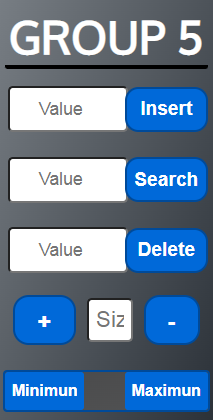
\includegraphics[width=0.2\textwidth]{img/avl_cap1.PNG}
        \caption{Panel de Control de AVL-Tree}
        \end{figure}

Las mismas operaciones que se encuentran en B-Tree tambien se realizan en AVL-Tree. 

Si en caso se desea eliminar un dato, se mostrará el siguiente mensaje:

        \begin{figure}[H]
        \centering
        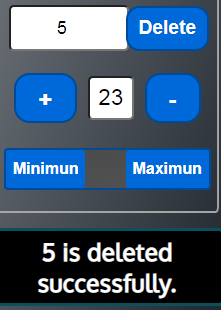
\includegraphics[width=0.2\textwidth]{img/avl_delet.PNG}
        \caption{Eliminacion en AVL-Tree}
        \end{figure}

   Y si se usa el boton SEARCH y se encuentra el dato, mostrará el mensaje de "found".

        \begin{figure}[H]
        \centering
        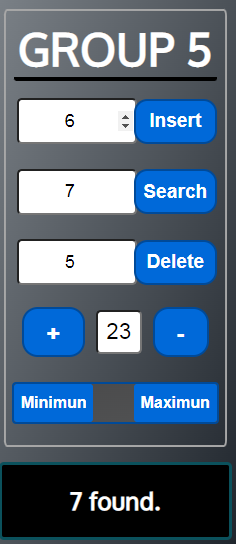
\includegraphics[width=0.2\textwidth]{img/avl_found.PNG}
        \caption{Busqueda en AVL-Tree}
        \end{figure}

        
\section{Resultados}


\subsection{B-Tree} 

Para B-Tree se puede desarrollar arboles de una manera facil utilizando la libreria P5.js .
Los botones + y - permiten aumentar y disminuir el tamaño del arbol para una mejor visualización.

        \begin{figure}[H]
        \centering
        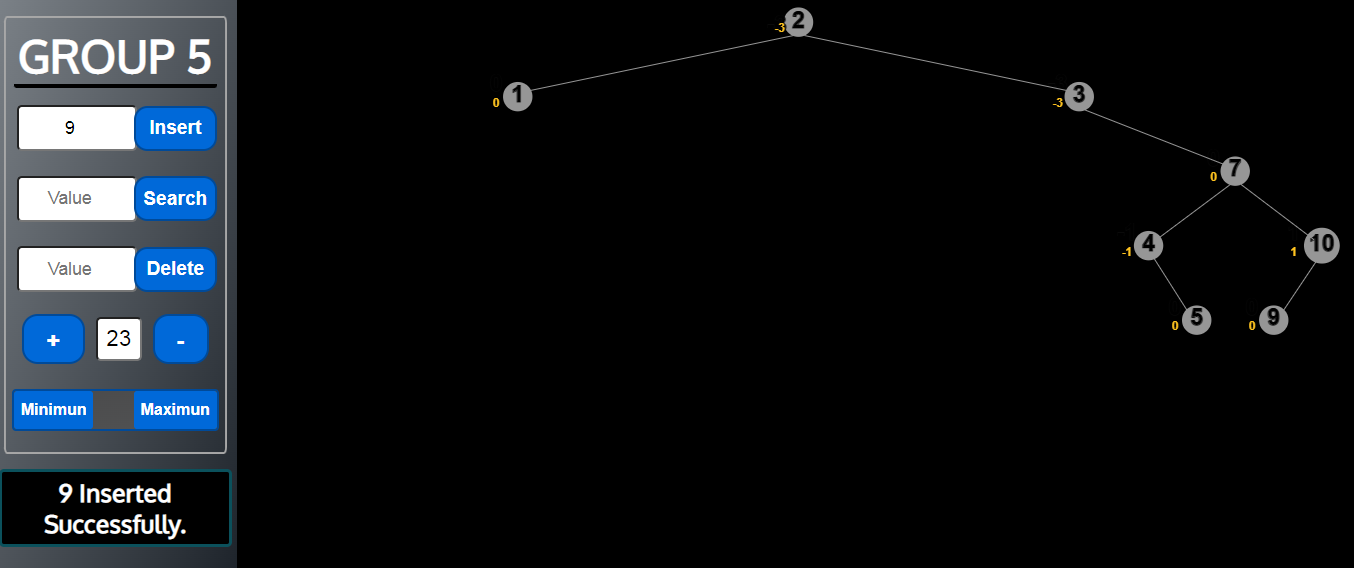
\includegraphics[width=0.8\textwidth]{img/btree_result.PNG}
        \caption{B-Tree en Heroku}
        \end{figure}

\subsection{AVL-Tree}


Para AVL-Treee  también se puede desarrollar arboles de una manera facil utilizando la libreria P5.js .
Los botones + y - permiten aumentar y disminuir el tamaño del arbol para una mejor visualización.

        \begin{figure}[H]
        \centering
        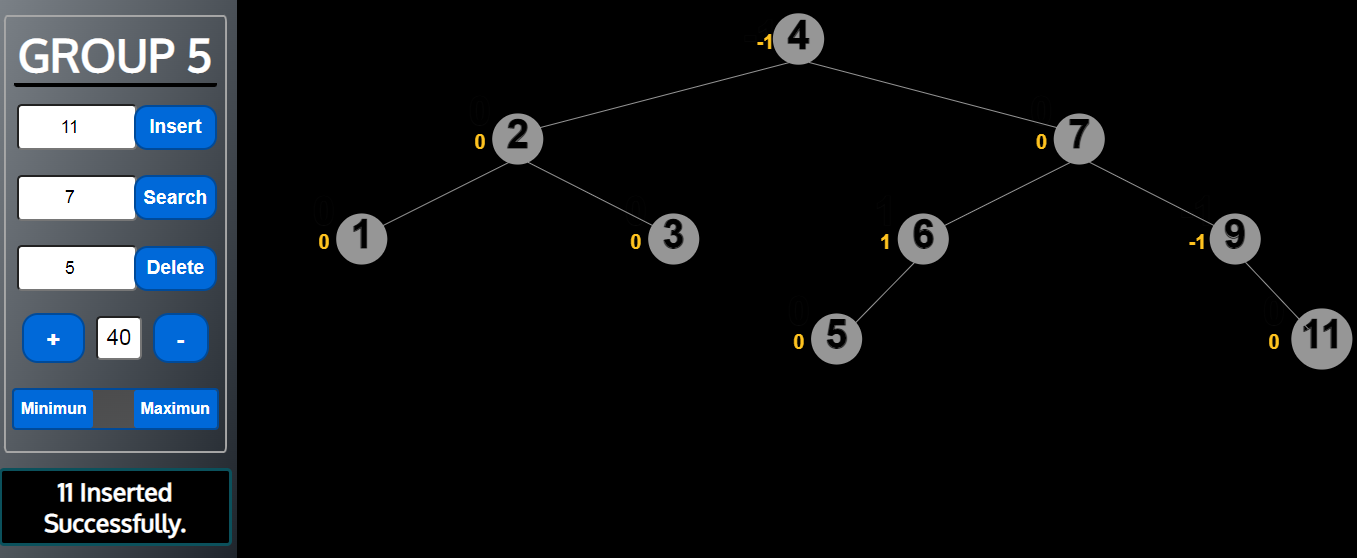
\includegraphics[width=0.8\textwidth]{img/avl_resultados.PNG}
        \caption{AVL-Tree en Heroku}
        \end{figure}

\section{Conclusiones}
    \subsection{B-Tree y AVL-Tree } 
    \begin{itemize}
        \item Logramos identificar que, entre las operaciones disponibles (Insert, Serach, Delete, Maximun y Minimun). Para AVL-Tree solo las operaciones de Insert y Delete necesitan ser balanceadas.
        \item Las aplicaciones nos permiten diferenciar  que para B-Tree no se balancea,  mientras que un AVL-Tree sí se balancea.
        \item Un AVL es más eficiente porque el balanceo nos permite asegurarnos que la complejidad simepre será nlog(n). Mientras que en el B-Tree se puede presentar el caso en que la complejidad llegue a "n" por no balancearse. 
       
    \end{itemize}

	
	
	\end{document}
